\documentclass[multi=tikzpicture,border=8pt]{standalone}
\usepackage[UTF8]{ctex}
\usepackage{amsmath,amssymb,tikz}
\usetikzlibrary{arrows.meta,calc}
\definecolor{blue}{HTML}{17365D}
\definecolor{red}{HTML}{AC3931}
\tikzset{every node/.style={font=\small},arrow/.style={-{Stealth[length=2.8mm]},thick},dim/.style={|<->|,thin},box/.style={draw,rounded corners,align=center,minimum width=2.5cm,minimum height=.8cm}}
\begin{document}
\begin{tikzpicture}

\draw[very thick](-2.5,0)--(2.5,0)node[right]{地面};\draw[fill=gray!15](-.15,0)--(0,.6)--(.15,0)--cycle;\draw[very thick,blue](-1.37477,0)--(1.37477,1.2);\fill[red](-1.37477,.08)circle(4pt)node[above left]{$M$};\fill[blue](1.37477,6)circle(4pt)node[above right]{$m$};\draw[arrow,blue](1.37477,5.7)--(1.37477,2.0);\draw[dim](2.3,0)--(2.3,6)node[right,midway]{$h$};\node[left]at(0,.6){$H$};\node[above]at(-1,1.9){$\sin\beta=2H/l$};

\end{tikzpicture}
\begin{tikzpicture}

\draw[very thick,blue](-2,-.8)--(2,.8);\fill(0,0)circle(2pt)node[below]{$O$};\draw[arrow,red](2,2.2)--(2,1)node[right]{$mu$};\draw[arrow,blue](2,.8)--(2.7,-.8)node[right]{$v_i$};\draw[arrow,blue](-2,-.8)--(-2.7,.8)node[left]{$v_i$};\node[below]at(0,-2){$ma u\cos\beta=(m+M)a v_i$};\node[above]at(0,2.8){关于支点的角动量守恒};

\end{tikzpicture}
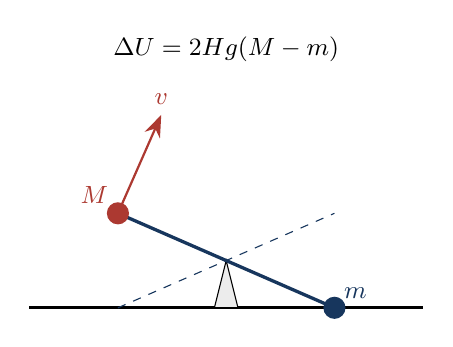
\begin{tikzpicture}

\draw[very thick](-2.5,0)--(2.5,0);\draw[fill=gray!15](-.15,0)--(0,.6)--(.15,0)--cycle;\draw[blue,dashed](-1.37477,0)--(1.37477,1.2);\draw[blue,very thick](-1.37477,1.2)--(1.37477,0);\fill[red](-1.37477,1.2)circle(4pt)node[above left]{$M$};\fill[blue](1.37477,0)circle(4pt)node[above right]{$m$};\draw[arrow,red](-1.37477,1.2)--(-0.82477,2.45)node[above]{$v$};\node[above]at(0,3){$\Delta U=2Hg(M-m)$};

\end{tikzpicture}
\begin{tikzpicture}
\draw[very thick](-2,0)--(2,0);\draw[very thick,red] plot coordinates {(-1.37477,1.20000) (-1.34700,1.26287) (-1.31923,1.32421) (-1.29145,1.38402) (-1.26368,1.44230) (-1.23591,1.49905) (-1.20813,1.55427) (-1.18036,1.60796) (-1.15259,1.66012) (-1.12481,1.71074) (-1.09704,1.75984) (-1.06927,1.80741) (-1.04149,1.85344) (-1.01372,1.89795) (-0.98595,1.94092) (-0.95817,1.98237) (-0.93040,2.02228) (-0.90263,2.06067) (-0.87486,2.09752) (-0.84708,2.13284) (-0.81931,2.16664) (-0.79154,2.19890) (-0.76376,2.22963) (-0.73599,2.25883) (-0.70822,2.28650) (-0.68044,2.31264) (-0.65267,2.33725) (-0.62490,2.36033) (-0.59712,2.38188) (-0.56935,2.40190) (-0.54158,2.42039) (-0.51380,2.43734) (-0.48603,2.45277) (-0.45826,2.46667) (-0.43048,2.47903) (-0.40271,2.48987) (-0.37494,2.49917) (-0.34716,2.50695) (-0.31939,2.51319) (-0.29162,2.51791) (-0.26385,2.52109) (-0.23607,2.52274) (-0.20830,2.52287) (-0.18053,2.52146) (-0.15275,2.51852) (-0.12498,2.51405) (-0.09721,2.50805) (-0.06943,2.50052) (-0.04166,2.49146) (-0.01389,2.48087) (0.01389,2.46875) (0.04166,2.45510) (0.06943,2.43991) (0.09721,2.42320) (0.12498,2.40496) (0.15275,2.38519) (0.18053,2.36388) (0.20830,2.34105) (0.23607,2.31668) (0.26385,2.29079) (0.29162,2.26336) (0.31939,2.23440) (0.34716,2.20392) (0.37494,2.17190) (0.40271,2.13835) (0.43048,2.10328) (0.45826,2.06667) (0.48603,2.02853) (0.51380,1.98886) (0.54158,1.94766) (0.56935,1.90493) (0.59712,1.86067) (0.62490,1.81488) (0.65267,1.76755) (0.68044,1.71870) (0.70822,1.66832) (0.73599,1.61641) (0.76376,1.56296) (0.79154,1.50799) (0.81931,1.45148) (0.84708,1.39345) (0.87486,1.33388) (0.90263,1.27279) (0.93040,1.21016) (0.95817,1.14601) (0.98595,1.08032) (1.01372,1.01310) (1.04149,0.94435) (1.06927,0.87407) (1.09704,0.80227) (1.12481,0.72893) (1.15259,0.65406) (1.18036,0.57766) (1.20813,0.49972) (1.23591,0.42026) (1.26368,0.33927) (1.29145,0.25675) (1.31923,0.17270) (1.34700,0.08711) (1.37477,0.00000)};\fill[red](-1.37477,1.2)circle(3pt)node[left]{发射};\fill[blue](1.37477,0)circle(3pt)node[above right]{落点};\draw[dim](-1.37477,-.6)--(1.37477,-.6)node[below,midway]{$l\cos\beta$};\node[above]at(0,3.2){$v_x=v\sin\beta,\ v_y=v\cos\beta$};
\end{tikzpicture}
\begin{tikzpicture}
\draw[arrow](0,0)--(6.3,0)node[right]{$\eta=m/(m+M)$};\draw[arrow](0,0)--(0,4.3)node[above]{$v^2/(2g)$};\draw[very thick,blue] plot coordinates {(1.50000,-0.46400) (1.53636,-0.42812) (1.57273,-0.39184) (1.60909,-0.35517) (1.64545,-0.31810) (1.68182,-0.28064) (1.71818,-0.24278) (1.75455,-0.20453) (1.79091,-0.16588) (1.82727,-0.12684) (1.86364,-0.08740) (1.90000,-0.04757) (1.93636,-0.00735) (1.97273,0.03327) (2.00909,0.07429) (2.04545,0.11570) (2.08182,0.15751) (2.11818,0.19971) (2.15455,0.24231) (2.19091,0.28530) (2.22727,0.32868) (2.26364,0.37246) (2.30000,0.41664) (2.33636,0.46121) (2.37273,0.50618) (2.40909,0.55154) (2.44545,0.59729) (2.48182,0.64344) (2.51818,0.68999) (2.55455,0.73693) (2.59091,0.78426) (2.62727,0.83199) (2.66364,0.88012) (2.70000,0.92864) (2.73636,0.97756) (2.77273,1.02687) (2.80909,1.07657) (2.84545,1.12667) (2.88182,1.17716) (2.91818,1.22805) (2.95455,1.27934) (2.99091,1.33102) (3.02727,1.38309) (3.06364,1.43556) (3.10000,1.48843) (3.13636,1.54169) (3.17273,1.59534) (3.20909,1.64939) (3.24545,1.70383) (3.28182,1.75867) (3.31818,1.81391) (3.35455,1.86954) (3.39091,1.92556) (3.42727,1.98198) (3.46364,2.03879) (3.50000,2.09600) (3.53636,2.15360) (3.57273,2.21160) (3.60909,2.27000) (3.64545,2.32878) (3.68182,2.38797) (3.71818,2.44755) (3.75455,2.50752) (3.79091,2.56789) (3.82727,2.62865) (3.86364,2.68981) (3.90000,2.75136) (3.93636,2.81331) (3.97273,2.87565) (4.00909,2.93839) (4.04545,3.00152) (4.08182,3.06505) (4.11818,3.12897) (4.15455,3.19329) (4.19091,3.25800) (4.22727,3.32311) (4.26364,3.38861) (4.30000,3.45451) (4.33636,3.52080) (4.37273,3.58749) (4.40909,3.65457) (4.44545,3.72204) (4.48182,3.78992) (4.51818,3.85818) (4.55455,3.92684) (4.59091,3.99590) (4.62727,4.06535) (4.66364,4.13520) (4.70000,4.20544) (4.73636,4.27608) (4.77273,4.34711) (4.80909,4.41853) (4.84545,4.49035) (4.88182,4.56257) (4.91818,4.63518) (4.95455,4.70819) (4.99091,4.78159) (5.02727,4.85538) (5.06364,4.92957) (5.10000,5.00416)};\draw[red,dashed](1.5,2.1)--(5.2,2.1);\fill(3.50253,2.1)circle(3pt)node[above left]{$\eta=0.58376$};\node[red]at(5.5,2.7){落点要求$0.525$ m};\node[below]at(3,-.8){$m/M\simeq1.4024$（图示初态模型）};
\end{tikzpicture}
\end{document}
